% set 0.5 inch indentation
\setlength{\parindent}{0.5in} 
% set paragraph space = 0 space
\setlength{\parskip}{0mm}
% set line space 1.5
\setlength{\baselineskip}{1.6em}

\chapter{LITERATURE REVIEW}
\label{ch:literature-review}
Write your introductory paragraph/s here (except for Chapter 1). Limit this section to two paragraphs. Follow the appropriate structure of writing paragraphs. Paragraphs should have at least four sentences. Paragraphs with more than 6 sentences must be split into two paragraphs.

\section{Section Name in Literature Review}
\label{section-name-in-literature-review}

\shortciteA{yamato92hmm} apply the background subtraction 
technique to extract blobs or human from a scene by the 
following conditions:
\[
\begin{array}{lc}
  {\rm if} & \left|{I_a (x,y) - I_b (x,y)}\right|< T,\;I_e (x,y) = 0 \\ 
  {\rm else} & I_e (x,y) = I_a (x,y), 
\end{array}
\]
where $I_e (x,y)$ is a human extracted image, $I_a (x,y)$ is an
original image, $I_b (x,y)$ is a background image, and $T$ is a
threshold. Figure~\ref{fig:mesh-feature} shows something. Some work also uses 
mesh features~\shortcite{yamato92hmm}.

% THE REASON ~ IS USED HERE BECAUSE WE TELL LATEX THAT THESE TWO WORDS SHOULD 
% GO TOGETHER IN THE SAME LINE.

\begin{figure}[h]
  \centering
  \caption[Mesh feature calculation]{Mesh feature calculation. Reprinted from the work of Yamato et al.\ (1992).}
  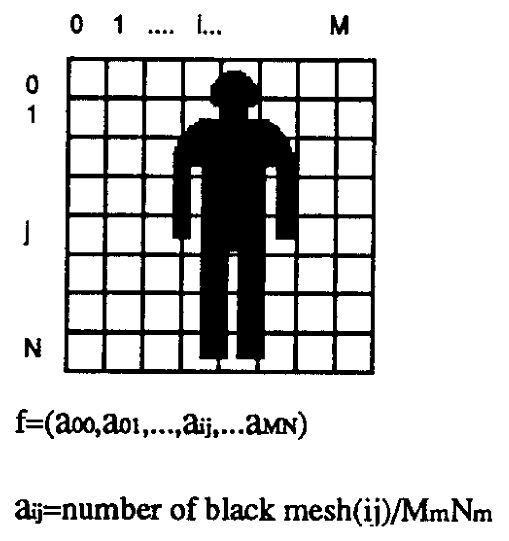
\includegraphics[width=2in]{figures/mesh-feature.jpg}  
  \label{fig:mesh-feature}
\end{figure}

\begin{table}[ht]
  \caption[Random Table 3]{Random Table 3}
  \begin{center}
    \begin{tabular}{cccc}
      \hline \textbf{v1} & \textbf{v2} & \textbf{v3} & \textbf{Overall} \\ \hline
        78.67\% & 87.33\% & 94.92\% & 85.64\% \\ \hline
    \end{tabular}
  \end{center}
  \label{tab:random_table_3}
\end{table} 

\section{Chapter Summary}
All chapters except Chapter 1 must include an introductory paragraph/s and a chapter summary.

\FloatBarrier